\documentclass[a4,12pt]{article}

% 畫圖
\usepackage{tikz}
\usetikzlibrary{automata,positioning,arrows}


% 排版
% \usepackage{enumerate}
% \newlist{steps}{enumerate}{1}
% \setlist[steps, 1]{label = Step \arabic*:}

% 中文插件
\usepackage{fontspec}
\usepackage{xeCJK}
\setCJKmainfont{Heiti TC}


% 插入圖片 using \includegraphics[scale = 1]{name.jpg}
\usepackage{graphicx}
\graphicspath{{./picture/}}
\usepackage{float} %设置图片浮动位置的宏包
\usepackage{subfigure}

% \usepackage[]{caption}
% \capto

\usepackage{multicol}

\title{Computer Graphics Hw 1} 
\author{賴柏勛 00957126}

\begin{document}
    \maketitle
    \section{操作方法}
    

    操作方式十分簡單,可以通過 menubar 的 type 決定現在使用的是哪個畫筆。
    
    Line、Rectangle、Circle 的操作方式都是類似的,使用滑鼠點拖,便可以拖出一個線段、矩形、圓形

    而 Point 則是直接點一下,便會在那個點畫出一個點,但因為實作的原因,所以大小固定為 1 bit。

    至於 Text ,則是在選擇 Text 畫筆後,通過鍵盤的輸入,便會在那個點畫出一個字母。

    Curve 更簡單,當按下滑鼠並拖動,就會畫出你滑鼠畫出的軌跡。

    而 Polygon 是通過點拖畫出多個線段,當到偵測滑鼠畫出的最後一個線段位置在第一個點時,便會自動將最後一個點與第一個點連起來,並根據模式去做填滿或畫線。

    Mode 的選擇就是選擇圖形是否要填滿,如果選擇 Fill ,則會填滿,如果選擇 line ,則會畫線。

    顏色的選擇則是通過三條華調來選擇,滑動的百分比便是顏色的強度,在滑條右邊也會預覽現在的顏色。
    
    Func 有三個按鈕,分別是 Gridline、Save Panel、Load Panel,按下 Gridline 就會根據現在 Gridline 的狀態來開關, Save Panel 的功能是將現在畫面的圖形儲存成一個起來, Load Panel 則是讀取剛剛存的圖形。
    
    最後,還有一個 New 的按鈕,可以清除畫布上的所有圖形。
    \section{心得}
    當看到這個題目時,我就決定要自己刻畫面上的 GUI 了,因為只是呼叫套件內容有點無聊,而且大部分的東西在範例程式已經撰寫得差不多了,身為資工人,這種有趣的東西就是要自己寫寫看,在 gui 的撰寫上,我發現通過 opengl 的函式,寫 gui 其實跟寫網站十分相似,只是需要去好好規劃每個物件的狀態,還有他們所遇到的事件,這次的作業我大概寫了三天左右,內容也只有 1000 行以內,應該是因為 Opengl 的函式庫方便好用,但是如果有機會的話,我也想用用看 Vulkan 寫這種小專案,感覺也很有趣。
    \section{實機畫面}
    \begin{figure}[H] 
    \centering
    
    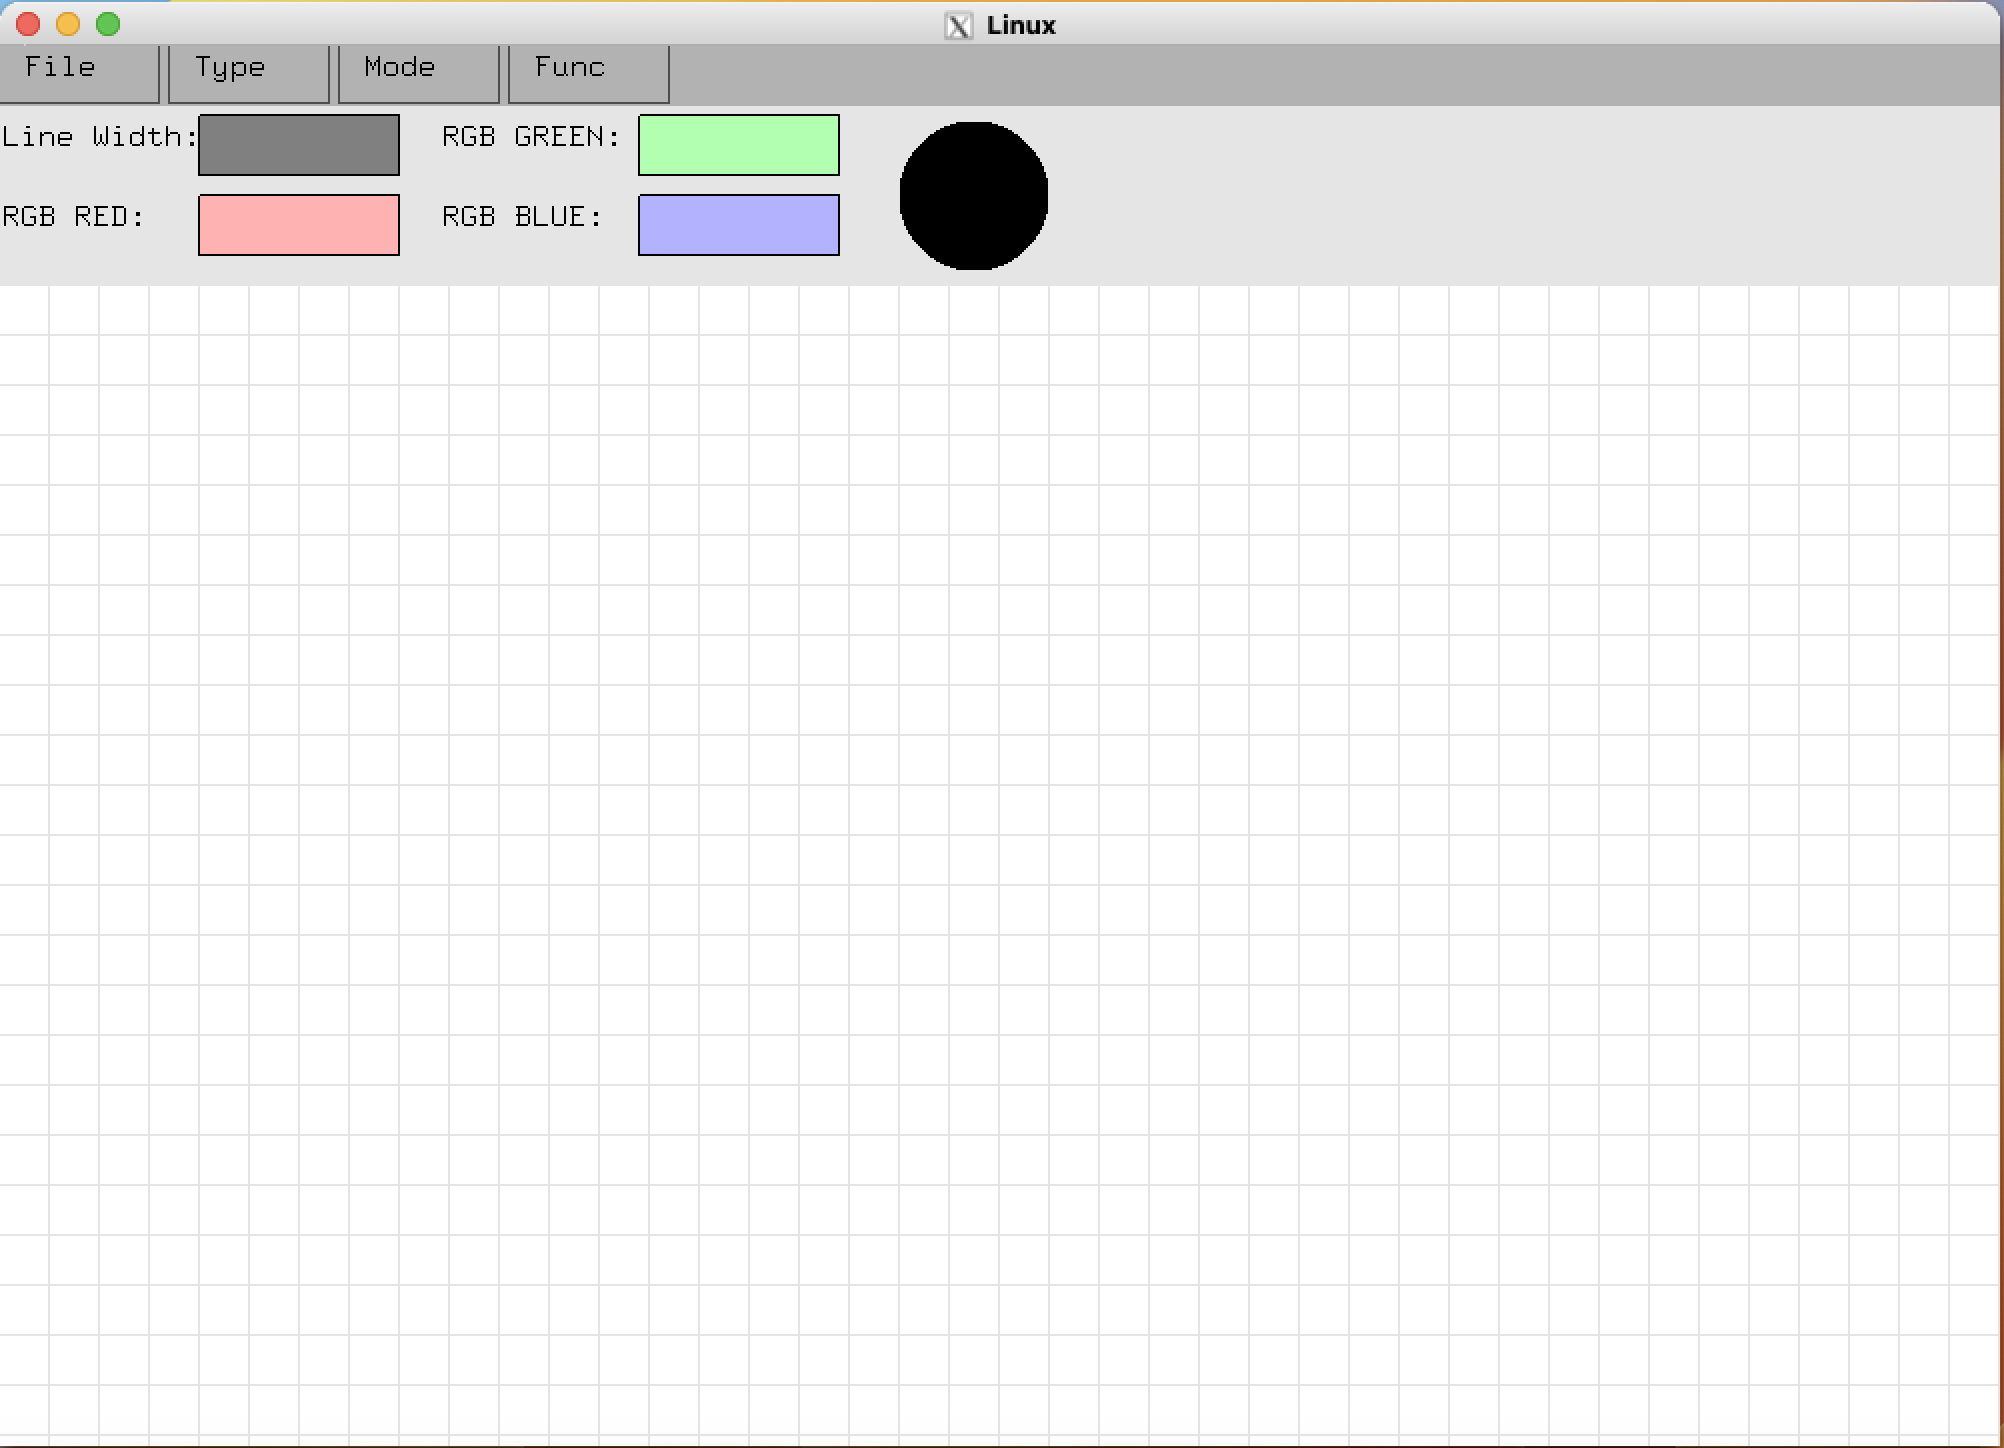
\includegraphics[scale = 0.3]{full.png}
    \caption{初始畫面}
    \end{figure}
    \begin{figure}[H] 
        \centering
       
    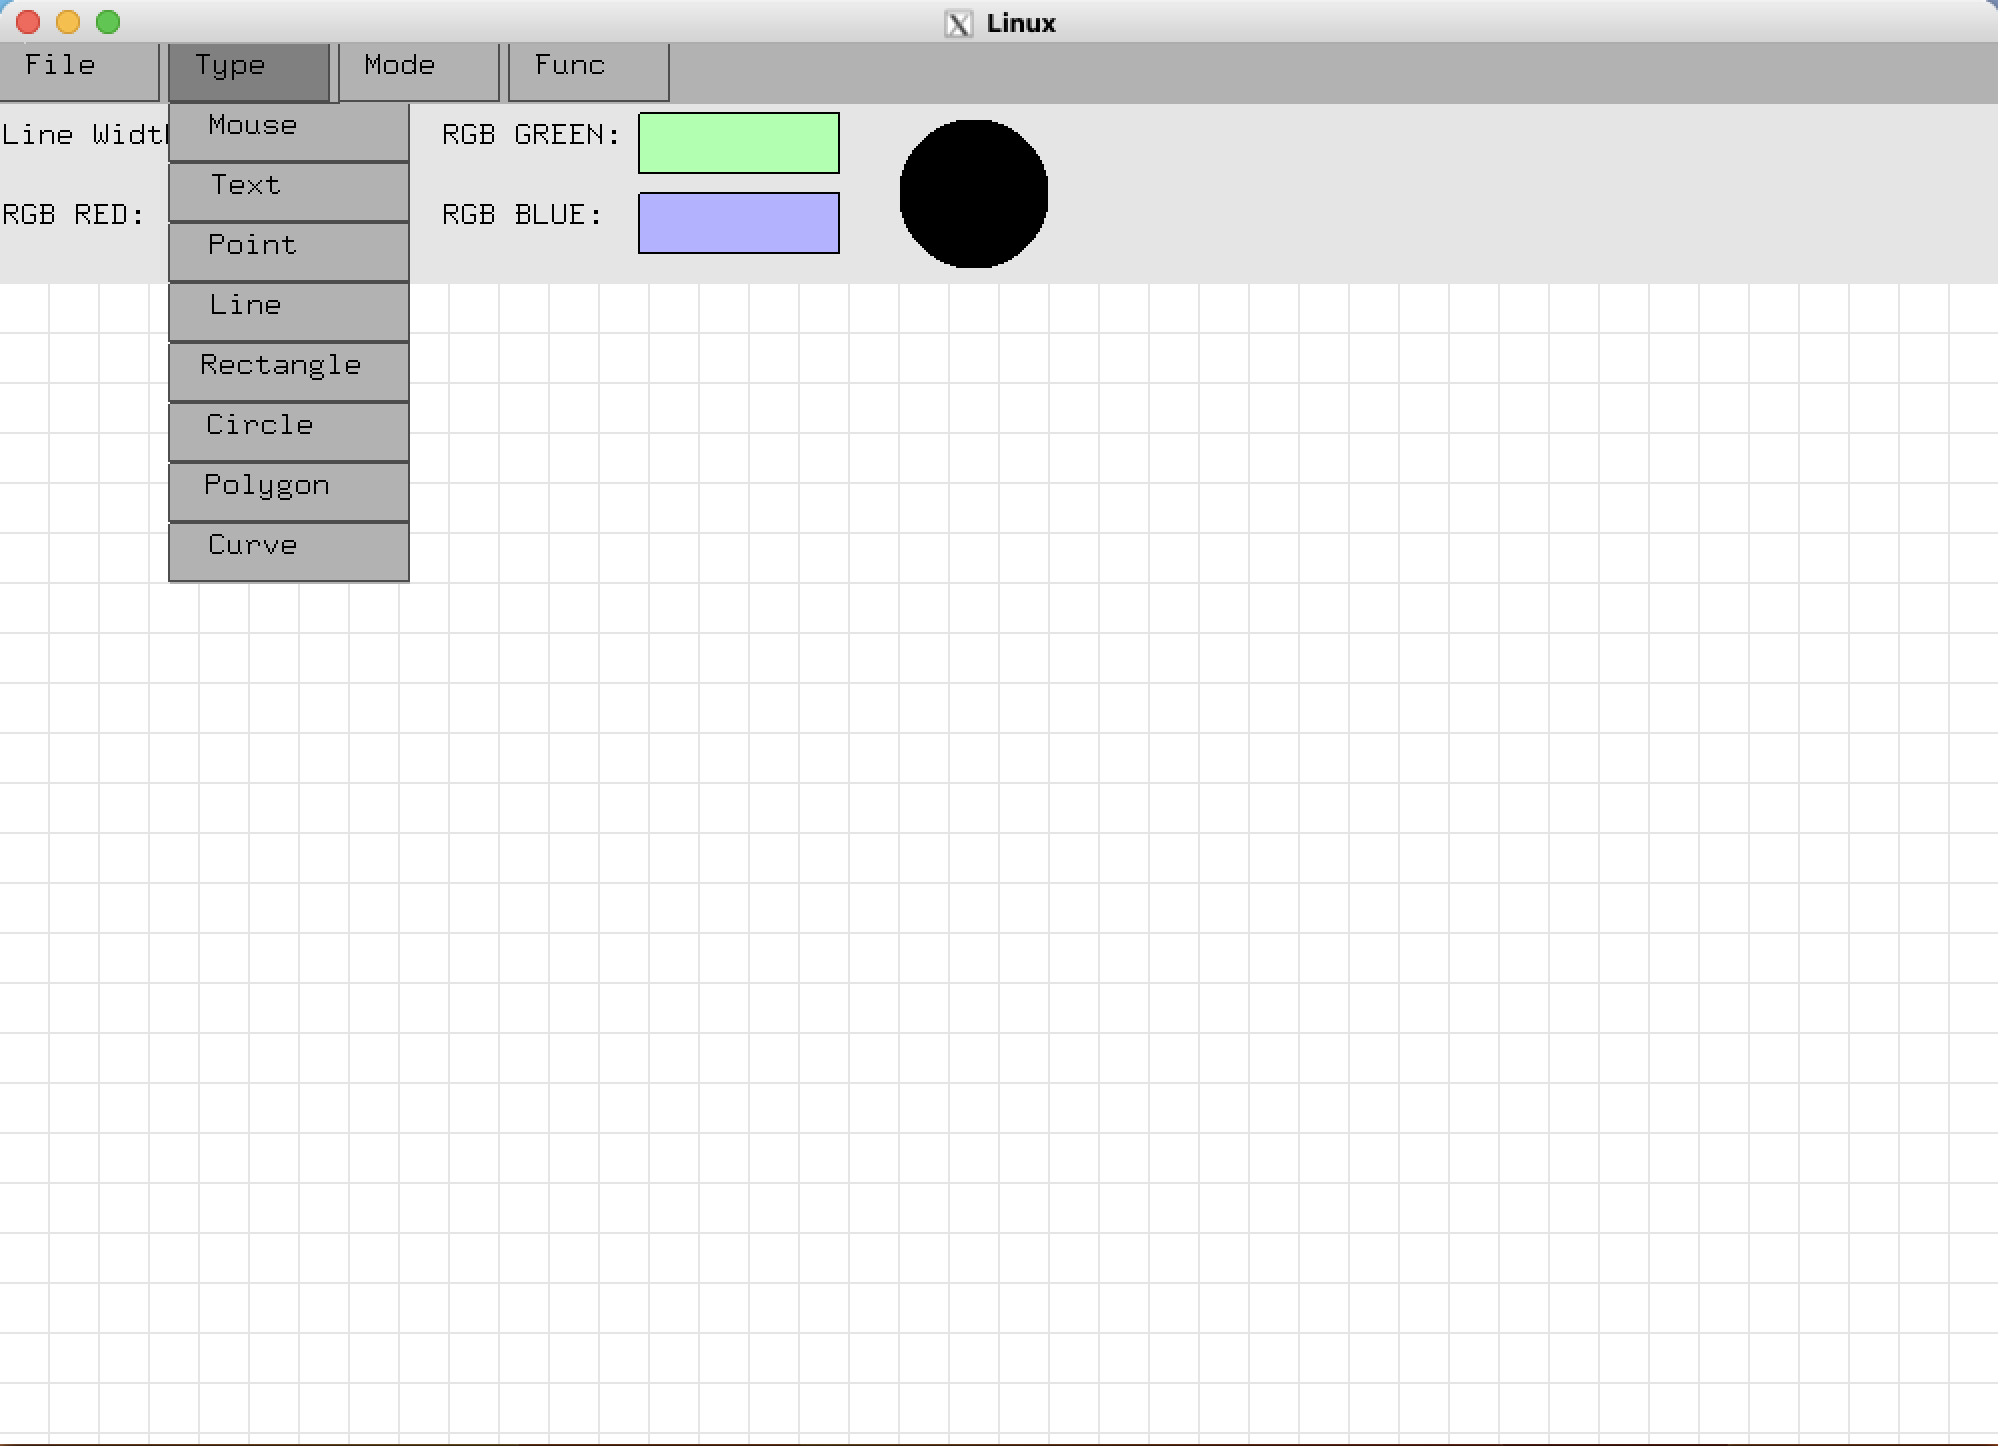
\includegraphics[scale = 0.3]{menubar.png}
    \caption{topbar}
    \end{figure}
    \begin{figure}[H] 
        \centering
       
    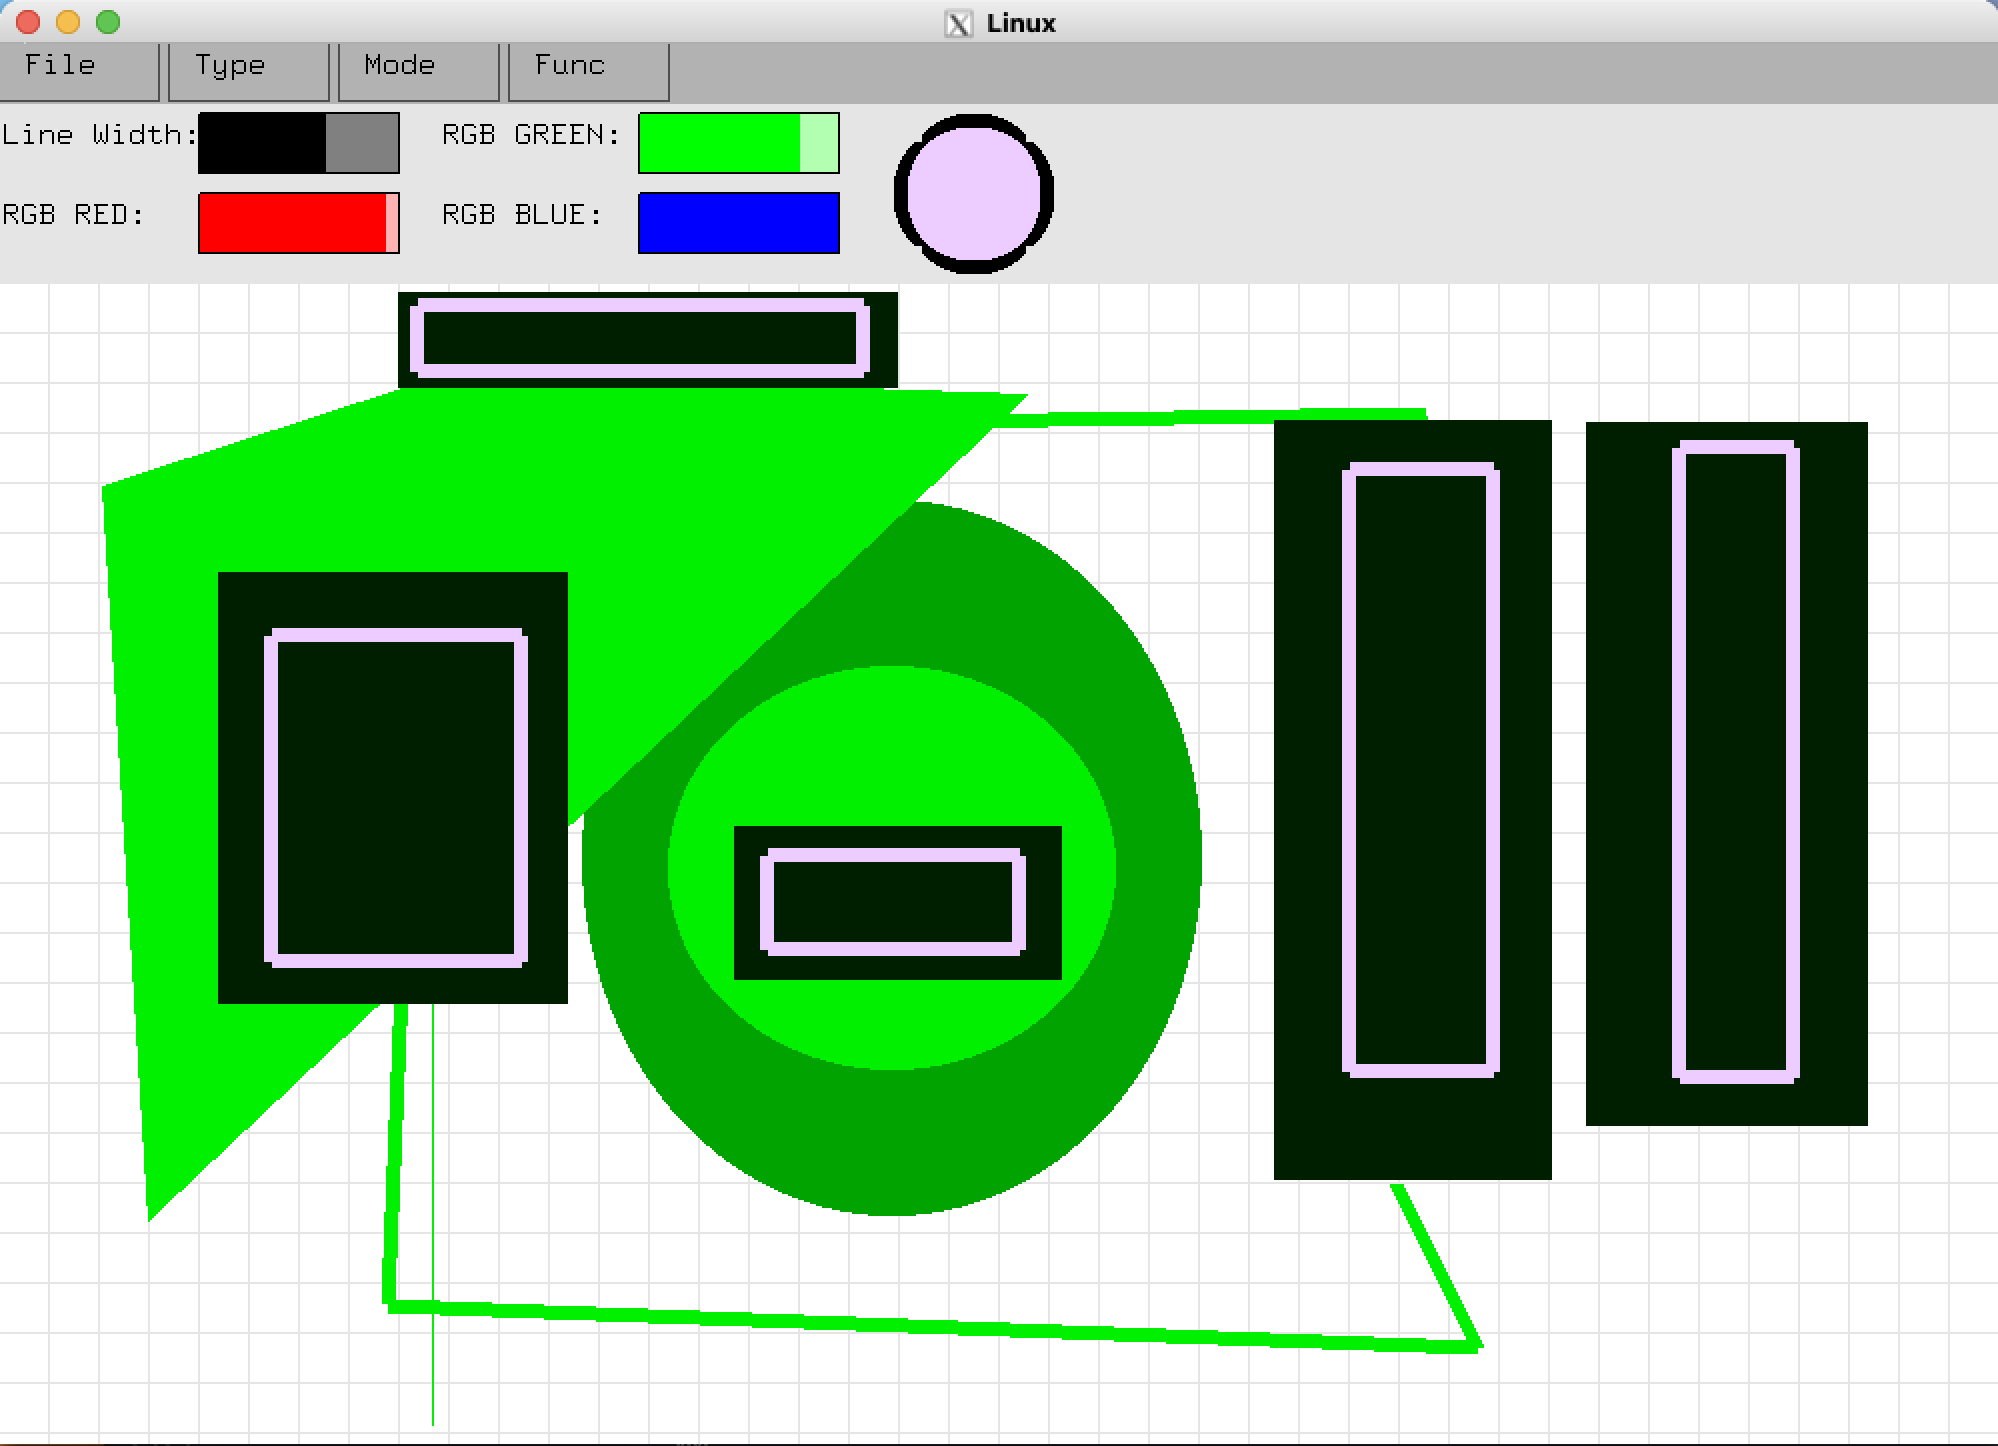
\includegraphics[scale = 0.3]{draw.png}
    \caption{實際畫出來}
\end{figure}
    \end{document}